\subsection{Budgeted Alarm Policies and Cross-Site Transport}

Figure~\ref{fig:budget} and Table~\ref{tab:e2} report the operational frontier for the prefix logistic scorer. On site A, raising the requested budget from 0.25 to 2 alarms per patient-day increases mean sensitivity from $0.185\pm0.061$ to $0.774\pm0.032$, while the realised alarm rate rises from $0.108\pm0.012$ to $1.366\pm0.026$. The realised rate stays below the requested budget at every operating point, which is the expected consequence of a finite-sample upper bound rather than evidence that the policy is slack by design. The tightest budget has the largest seed-to-seed sensitivity variance, because a small change in the calibrated threshold moves several of the 168 eligible A events across the detection boundary. Median lead time among detected events stays between 8.7 and 10 hours, but this conditional median must be read with the corresponding sensitivity: it describes only the events that were detected.

\begin{figure}[tb]
\centering
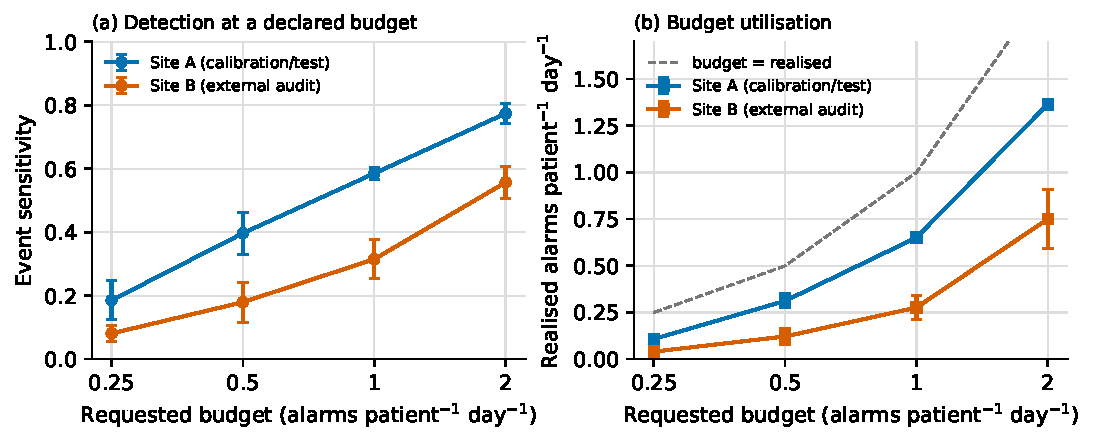
\includegraphics[width=\linewidth]{figures/e2_budget.pdf}
\caption{Three-seed E2 operating curves for the prefix logistic scorer. (a) Event sensitivity versus the requested patient-average alarm budget. (b) Realised alarm rate versus the requested budget; the dashed diagonal marks exact budget utilisation. Error bars are sample standard deviations over seeds 0--2. Site B uses the A-calibrated threshold without target labels.}
\label{fig:budget}
\end{figure}

\begin{table}[tb]
\centering
\caption{E2 budget sweep for the prefix logistic scorer, mean $\pm$ sample standard deviation over three seeds. Rates are alarms per patient-day; lead time is the median among detected events in hours; violation is the fraction of test patients whose per-day count exceeds the budget. The 4- and 8-per-day rows coincide because the threshold grid reaches its floor.}
\label{tab:e2}
\small
\begin{tabular}{lcccc}
\toprule
\multicolumn{5}{c}{Site A (calibration/test)} \\
Budget & Rate & Sens. & Lead & Viol. \\
\midrule
0.25 & $0.108\pm0.012$ & $0.185\pm0.061$ & $9.5\pm0.5$ & $0.074\pm0.001$ \\
0.50 & $0.312\pm0.037$ & $0.397\pm0.067$ & $8.7\pm0.6$ & $0.151\pm0.014$ \\
1.00 & $0.651\pm0.022$ & $0.585\pm0.020$ & $9.3\pm0.6$ & $0.210\pm0.003$ \\
2.00 & $1.366\pm0.026$ & $0.774\pm0.032$ & $10.0\pm0.0$ & $0.309\pm0.004$ \\
4.00 & $2.096\pm0.026$ & $0.894\pm0.011$ & $10.0\pm0.0$ & $0.271\pm0.012$ \\
\bottomrule
\end{tabular}

\vspace{6pt}
\begin{tabular}{lcccc}
\toprule
\multicolumn{5}{c}{Site B (external audit)} \\
Budget & Rate & Sens. & Lead & Viol. \\
\midrule
0.25 & $0.040\pm0.014$ & $0.081\pm0.026$ & $8.5\pm0.5$ & $0.030\pm0.010$ \\
0.50 & $0.122\pm0.044$ & $0.180\pm0.063$ & $8.2\pm0.3$ & $0.065\pm0.023$ \\
1.00 & $0.276\pm0.063$ & $0.315\pm0.062$ & $8.3\pm0.6$ & $0.094\pm0.025$ \\
2.00 & $0.750\pm0.157$ & $0.557\pm0.051$ & $9.0\pm0.0$ & $0.163\pm0.038$ \\
4.00 & $1.473\pm0.250$ & $0.724\pm0.049$ & $9.3\pm0.6$ & $0.131\pm0.025$ \\
\bottomrule
\end{tabular}
\end{table}

The external audit exposes a qualitatively different operating point. At the 1-per-day budget the A-calibrated policy emits $0.276\pm0.063$ alarms per B patient-day, less than half the A rate, and detects $0.315\pm0.062$ of eligible B events compared with $0.585\pm0.020$ at A. At the tightest budget, B sensitivity falls to $0.081\pm0.026$ while the realised B alarm rate is only $0.040\pm0.014$. The direction of the rate change is not a free lunch: the same threshold is simply less active on the shifted score distribution, and the lost activity is concentrated on true events. This is exactly the failure mode that a threshold-only transport claim would hide, and it is consistent with recent evidence that score distributions and calibration can shift across hospitals \citep{lu2022estimating,wu2026outofdistribution}. A target-site calibration study is therefore a separate deployment step, not an optional refinement.

The deliberately invalid timestep comparator is less conservative at the two tightest budgets. At budget 0.25 it selects threshold 0.0445 instead of 0.0543, raises the A alarm rate from 0.117 to 0.183, raises A sensitivity from 0.250 to 0.321, and raises the patient-violation fraction from 0.074 to 0.115. At budget 0.50 it selects 0.0297 instead of 0.0346, raises the alarm rate from 0.328 to 0.450, raises sensitivity from 0.452 to 0.512, and raises the violation fraction from 0.161 to 0.214. At budgets of 1 and above the finite grid selects the same threshold for both procedures on this split, so the comparator is not a universal ranking. The result is nevertheless the expected qualitative signature of effective-sample-size inflation: the timestep procedure buys sensitivity by shrinking its guard band and paying for it in per-patient budget violations.

The GRU changes the level of the frontier but not its transport behaviour. At 1 alarm per patient-day its seed-0 A sensitivity is 0.685 and its B sensitivity is 0.326, compared with 0.607 and 0.382 for the logistic model. At 0.25 per day the GRU reaches 0.393 at A and 0.129 at B. The GRU therefore looks better than logistic at the tight internal budget and at the moderate internal budget, but worse at the external 1-per-day point; the ordering is not stable across sites. This is a useful negative result for architecture-centred claims: a more expressive scorer can move the internal frontier without repairing the site shift. It also reinforces that the calibration procedure, not the backbone alone, determines whether a stated alert budget is met.

Two limitations of the grid are visible in the table. First, the 4- and 8-per-day rows are identical because the threshold grid stops at 0.01; above roughly 2 alarms per patient-day the budget constraint is no longer binding and the frontier is truncated by the candidate set. Second, every certified operating point has a realised rate below its requested budget, so the experiment demonstrates conservative risk control rather than tight budget utilisation. Neither observation undermines the certificate, but both matter for engineering deployment: a hospital that needs a precise alarm load may prefer a finer grid or a utility-based selection among certified thresholds, and a hospital that needs a higher sensitivity must accept the corresponding increase in realised alert volume. The clinical interpretation of these rates also depends on local workflow and alarm-fatigue tolerance, which this retrospective study does not measure \citep{ray2026alert,jaidev2026sepsis}.
